\documentclass[aspectratio=169,11pt]{beamer}
\usepackage{fontspec}
\setsansfont{Arial}
\usepackage{graphicx}
\graphicspath{{figuras_avances/}}

\setbeamertemplate{navigation symbols}{}
\setbeamertemplate{footline}{\hfill{\scriptsize\color{tinta2}\insertframenumber}\hspace{3mm}\vspace{2mm}}
\definecolor{tinta}{HTML}{1F1F1E}
\definecolor{tinta2}{HTML}{5C5C58}
\definecolor{acento}{HTML}{2A78D6}
\setbeamercolor{frametitle}{fg=tinta}
\setbeamercolor{title}{fg=tinta}
\setbeamercolor{subtitle}{fg=tinta2}
\setbeamercolor{normal text}{fg=tinta}
\setbeamercolor{itemize item}{fg=acento}
\setbeamerfont{frametitle}{size=\large,series=\bfseries}
\setbeamertemplate{itemize items}[circle]
\setbeamertemplate{frametitle}{\vspace{2mm}\insertframetitle\vspace{-1mm}}
\setbeamersize{text margin left=7mm,text margin right=7mm}

% pie de figura: descriptivo, una o dos líneas
\newcommand{\pie}[1]{\par\vspace{0.5mm}{\raggedright\scriptsize\color{tinta2}#1\par}}
% figura que ocupa el ancho de la diapositiva
\newcommand{\figura}[1]{{\centering\includegraphics[width=\textwidth,height=0.78\textheight,keepaspectratio]{#1}\par}}
\newcommand{\bh}{$\hat\beta$}

\title{Actuador con recorte, x0 entrenable\\y referencia black-box}
\subtitle{Avances del modelo gray-box de Wilson-Cowan}
\date{}
\author{}

\begin{document}

\begin{frame}
  \titlepage
\end{frame}

\begin{frame}{Resumen}
  \vspace{2mm}
  \begin{itemize}\setlength\itemsep{2.5mm}
    \item El actuador pasó de $3\tanh(P_f/3)$ a un recorte duro en $\pm 3$, con el mismo filtro de 1~ms (e21).
    \item Con el recorte, el estado de filtro recupera \bh{} con 0,5\,\% de error con $\sigma = 0{,}01$.
    \item x0 entrenable baja el error de \bh{} del estado de filtro de 10,3 a 1,4\,\% con $\sigma = 0{,}05$ (e23). En las correcciones con red no lo baja (e22).
    \item En lazo cerrado se mide la distancia al lazo de la planta. Con el nivel de saturación de diseño y x0 entrenable, el estado de filtro reproduce el lazo de la planta con los dos niveles de ruido.
    \item Una Neural ODE black-box con historia del comando iguala a la corrección con historia de 5~ms y queda detrás de las formas estructuradas (e24).
  \end{itemize}
  \vfill
  \pie{Salvo aclaración, cada valor es la media de tres semillas. NRMSE sobre los 13 escenarios de test que interpolan. $\sigma$ es el desvío del ruido de medición.}
\end{frame}

\begin{frame}{Forma de la saturación del actuador}
  \begin{columns}[c]
    \begin{column}{0.57\textwidth}
      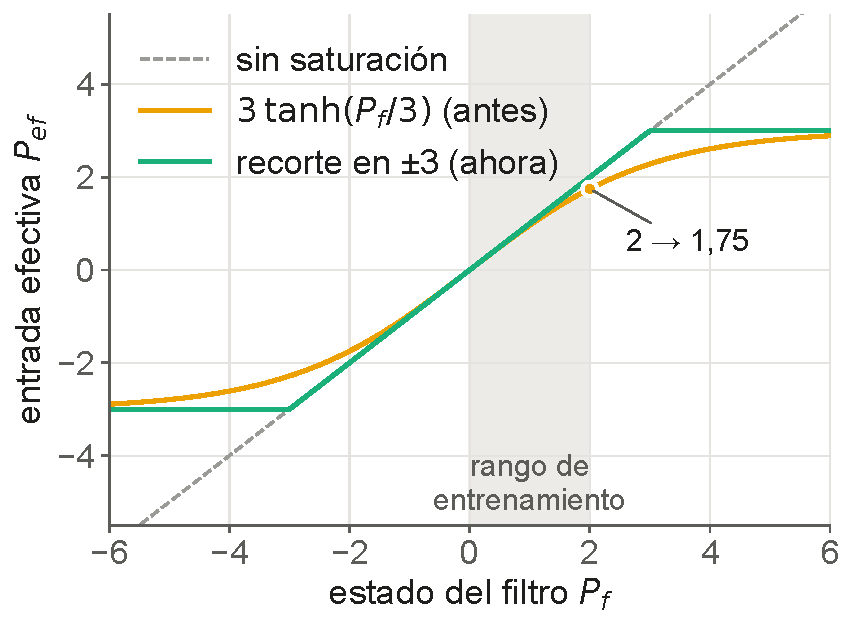
\includegraphics[width=\linewidth]{saturacion.pdf}
      \pie{Entrada efectiva en función del estado del filtro. La franja gris es el rango de comandos de entrenamiento.}
    \end{column}
    \begin{column}{0.4\textwidth}
      \small
      \begin{itemize}\setlength\itemsep{2mm}
        \item La tanh comprime por debajo del nivel. Un comando de 2 sale como 1,75 y uno de 3 como 2,28.
        \item El recorte es lineal hasta $\pm 3$.
        \item Los datos de entrenamiento no llegan a 3, así que el nivel no se identifica.
        \item En lazo cerrado el controlador pide comandos de hasta $\pm 11$.
      \end{itemize}
    \end{column}
  \end{columns}
\end{frame}

\begin{frame}{Error de \bh{} con tanh y con recorte}
  \figura{beta_tanh_vs_recorte.pdf}
  \pie{Error medio de los diez parámetros en la planta con actuador, con tanh (e16) y con recorte (e21). Redes con warm start desde el white-box. La agnóstica con tanh tiene una sola semilla.}
\end{frame}

\begin{frame}{NRMSE con tanh y con recorte}
  \figura{nrmse_tanh_vs_recorte.pdf}
  \pie{NRMSE de test de los mismos modelos. Con la tanh la compresión quedaba absorbida en $w_{EE}$, $w_{EI}$ y $a_e$, con NRMSE parecido y \bh{} peor.}
\end{frame}

\begin{frame}{Capacidad de cada red con $\beta$ verdadero fijo (e20)}
  \begin{columns}[c]
    \begin{column}{0.6\textwidth}
      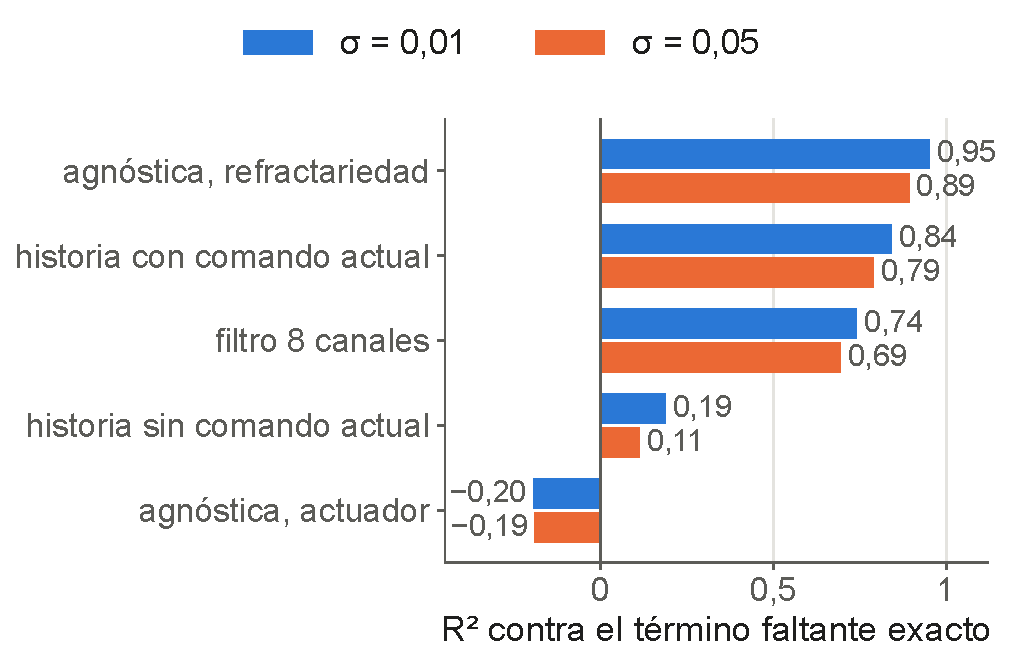
\includegraphics[width=\linewidth]{beta_verdadero_r2.pdf}
      \pie{R² de la red contra el término faltante exacto, con $\beta$ fijo en el valor verdadero. Primera fila, refractariedad. Las demás, actuador con tanh.}
    \end{column}
    \begin{column}{0.37\textwidth}
      \small
      \begin{itemize}\setlength\itemsep{2mm}
        \item Sin el comando actual, la red no reconstruye el estado del filtro.
        \item Con $\beta$ libre la historia pasada parecía equivalente a la de 5~ms, porque \bh{} absorbía parte del término.
        \item La historia pasada queda solo como planta.
      \end{itemize}
    \end{column}
  \end{columns}
\end{frame}

\begin{frame}{x0 entrenable sobre el actuador con recorte}
  \figura{x0_entrenable_beta.pdf}
  \pie{Error de \bh{} antes (gris) y después (azul) de la segunda etapa con el estado inicial de cada ventana entrenable. Redes en e22, estado de filtro en e23, desde el checkpoint de e21.}
\end{frame}

\begin{frame}{Lazo cerrado sobre la planta y sobre cada modelo}
  \figura{trazas_lazo.pdf}
  \pie{$E$ y comando $P$ con el controlador IMC del paper, referencia theta-gamma, entre 1500 y 1700~ms. Planta con recorte, semilla 0, $\sigma = 0{,}01$. La franja gris marca $\pm 3$.}
\end{frame}

\begin{frame}{Distancia entre el lazo con el modelo y el lazo con la planta}
  \figura{distancia_lazos.pdf}
  \pie{Distancia eficaz en $E$ e $I$ al lazo con el simulador, último 80\,\% de la corrida. Mediana de tres semillas, planta con recorte.}
\end{frame}

\begin{frame}{Seguimiento y distancia}
  \begin{columns}[c]
    \begin{column}{0.58\textwidth}
      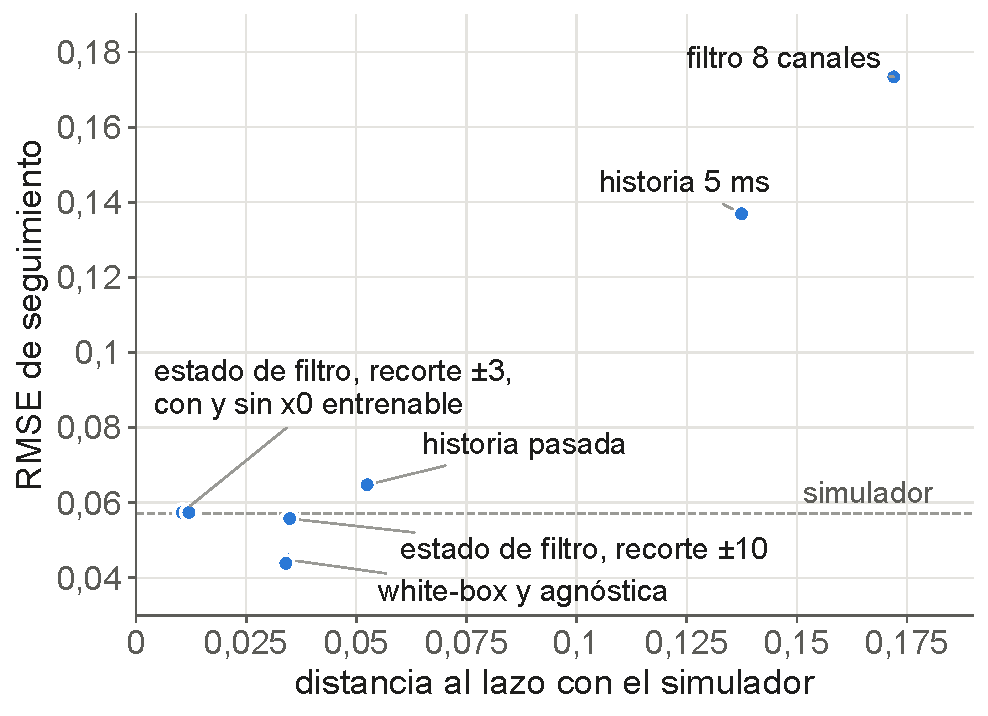
\includegraphics[width=\linewidth]{rmse_vs_distancia.pdf}
      \pie{RMSE de seguimiento contra distancia al lazo con la planta, theta-gamma, $\sigma = 0{,}01$. Línea punteada, RMSE con la planta.}
    \end{column}
    \begin{column}{0.39\textwidth}
      \small
      \begin{itemize}\setlength\itemsep{2mm}
        \item El white-box y la agnóstica siguen mejor que la planta, con lazos lejanos al de la planta.
        \item El RMSE de seguimiento no ordena modelos. Se reporta junto con la distancia.
        \item Con el comando dentro del rango de entrenamiento, el estado de filtro, el white-box y la agnóstica quedan a menos de 0,003.
      \end{itemize}
    \end{column}
  \end{columns}
\end{frame}

\begin{frame}{Estado de filtro en el lazo: nivel de saturación y x0}
  \figura{estado_filtro_en_lazo.pdf}
  \pie{Distancia al lazo con la planta para el estado de filtro. * Planta con filtro y sin saturación, modelo sin recorte. Filas con x0 entrenable de e23, las demás de e21.}
\end{frame}

\begin{frame}{Referencia black-box (e24)}
  \figura{black_box.pdf}
  \pie{NRMSE de test de la Neural ODE black-box $\dot x = g(I, E, P, Q)$ y de la misma red con historia del comando de 5~ms. Red de 64 unidades, 3000 épocas, desde cero.}
\end{frame}

\begin{frame}{Síntesis}
  \vspace{2mm}
  \begin{itemize}\setlength\itemsep{2.5mm}
    \item El recorte deja una sola no linealidad en el actuador, y con ella el estado de filtro identifica $\beta$.
    \item El error de \bh{} tiene dos fuentes. El ruido en las condiciones iniciales se corrige con x0 entrenable. La falta del estado del filtro en las redes no se corrige con x0.
    \item La precisión en lazo abierto no alcanza para elegir un modelo para control. La distancia entre lazos separa los modelos.
    \item El nivel de saturación tiene que venir del diseño o de un ensayo con comandos grandes. Con ese nivel y x0 entrenable, el lazo con el modelo coincide con el de la planta con $\sigma = 0{,}01$ y con $\sigma = 0{,}05$.
    \item En lazo abierto la black-box con historia iguala a la corrección con red. La ventaja del gray-box está en los parámetros identificables y en las formas estructuradas.
  \end{itemize}
\end{frame}

\begin{frame}{Pendientes}
  \vspace{2mm}
  \begin{itemize}\setlength\itemsep{2.5mm}
    \item Llevar la black-box al lazo cerrado.
    \item Declarar en Métodos la excepción al warm start de la black-box y la línea de saturación de e19.
    \item Unificar la métrica de 13 y de 14 escenarios.
    \item Decidir el alcance de la planta con las dos perturbaciones juntas.
    \item Actualizar el documento del controlador con el recorte y la distancia entre lazos.
    \item Decidir qué migra al repositorio limpio. e22, e23, e24 y la planta sin saturación están solo en el de trabajo.
  \end{itemize}
\end{frame}

\end{document}
